\documentclass[12pt]{article}
\usepackage{scrextend}
\usepackage[utf8]{inputenc}
\usepackage[polish]{babel}
\usepackage[T1]{fontenc}%polskie znaki
\usepackage[utf8]{inputenc}%polskie znaki
\usepackage{geometry}
\usepackage{float}
\usepackage{enumitem}
\usepackage{hyperref}
\usepackage{graphicx}
\usepackage{tabulary}
\usepackage{etoc}
\usepackage[normalem]{ulem} 
\usepackage{tikz}
\usepackage[bf]{caption}
\usepackage{listings}
\renewcommand{\baselinestretch}{1.5}

\usepackage{listings}
\usepackage{xcolor}
 
\definecolor{codegreen}{rgb}{0,0.6,0}
\definecolor{codegray}{rgb}{0.5,0.5,0.5}
\definecolor{codepurple}{rgb}{0.58,0,0.82}
\definecolor{backcolour}{rgb}{0.95,0.95,0.92}
 
\lstdefinestyle{mystyle}{
    backgroundcolor=\color{backcolour},   
    commentstyle=\color{codegreen},
    keywordstyle=\color{magenta},
    numberstyle=\tiny\color{codegray},
    stringstyle=\color{codepurple},
    basicstyle=\ttfamily\footnotesize,
    breakatwhitespace=false,         
    breaklines=true,                 
    captionpos=b,                    
    keepspaces=true,                 
    numbers=left,                    
    numbersep=5pt,                  
    showspaces=false,                
    showstringspaces=false,
    showtabs=false,                  
    tabsize=2,
    postbreak=\mbox{\textcolor{red}{$\hookrightarrow$}\space}
}
\renewcommand{\lstlistlistingname}{Spis listingów}\lstset{style=mystyle}

\graphicspath{ {img/} }
\newgeometry{lmargin=2.0cm, rmargin=2.0cm, tmargin=2.0cm, bmargin=2.0cm}
\clubpenalty=9996
\widowpenalty=9999
\brokenpenalty=4991
\predisplaypenalty=10000
\postdisplaypenalty=1549
\displaywidowpenalty=1602

\title{ 
    \vspace*{55mm}
    \textsc{
        \textbf{Urządzenia Peryferyjne}\\
        \large Sprawozdanie  \\
        \Large Analizator parametrów sieci
        }
} 
\author{
Damian Koper,  241292\\
Wiktor Pieklik, 241282\\
}

\date{\today}

\begin{document}
\maketitle


\newpage
\setcounter{tocdepth}{2}
\localtableofcontents
\listoffigures
\lstlistoflistings

\newpage

\section{Cel ćwiczenia}
Celem ćwiczenia było zapoznanie się z urządzeniem służącym do analizy parametrów sieciowych używanym w automatyce. Na zajęciach dostępny był analizator parametrów sieci EMA-90N firmy Contrel, który umożliwia kontrolę stanu sieci elektrycznej poprzez mierzenie parametrów takich jak: napięcie, prąd, moc czynna, moc bierna, cos(fi), harmoniczne prądu i inne. Urządzenie umożliwia komunikację za pomocą Ethernet przy wykorzystaniu protokołu modbus.
\section{Podstawowe zagadnienia związane z siecią elektryczną}
% Ogólna definicja
\subsection{Napięcie}
Napięcie elektryczne - to różnica potencjałów między dwoma punktami obwodu elektrycznego. Symbolem napięcia jest \textit{U}, a samo napięcie wyraża się w Voltach [V].\\
Napięcie można również wyrazić jako stosunek pracy wykonanej przeciwko polu, podczas przenoszenia ładunku elektrycznego między punktami, dla których określa się napięcie, do wartości tego ładunku. Określa to wzór:\\
\begin{equation}
    U_{AB} = \varphi_B - \varphi_A = \frac{W_{A \rightarrow B}}{q}
\end{equation}
\subsubsection{Napięcie sieciowe}
Napięcie sieciowe – napięcie elektryczne występujące w sieci niskiego napięcia danego kraju. Napięcie sieciowe ma charakterystykę sinusoidalną i w zależności od kraju: częstotliwość 50 lub 60 Hz i napięcie od 100 do 240 V (w Polsce 230 V / 50 Hz – określa to Polska Norma PN-IEC 60038). Większość urządzeń powszechnego użytku jest zasilana z wykorzystaniem napięcia sieciowego lub napięciem przetworzonym z napięcia sieciowego, przy użyciu transformatorów napięcia. Należy zaznaczyć, że wartość 230 V to wartość skuteczna napięcia przemiennego. Przy 230 V szczytowa wartość napięcia sieciowego wynosi $230 V * \sqrt{2} = 325 V$. Dopuszczalne odchylenia wynoszą $\pm\ 10\%$, czyli od 207 do 253 V.
\subsection{Prąd}
Prąd elektryczny - to uporządkowany ruch ładunków elektrycznych. Nośnikami tych ładunków mogą być elektrony lub jony.\\
Ściśle związaną jednostką z prądem jest \textbf{natężenie prądu}, czyli wielkość fizyczna charakteryzująca przepływ prądu elektrycznego zdefiniowana jako stosunek wartości przepływającego ładunku elektrycznego do czasu przepływu tego ładunku.
Symbolem natężenia prądu elektrycznego jest \textit{I} i wyrażane jest w Amperach [A]. Natężenie prądu określa się wzorem:
\begin{equation}
    I = \frac{\partial{q}}{\partial{t}},
\end{equation}
Gdzie:
    \begin{itemize}[noitemsep]
        \item $\partial{q}$ - zmiana ładunku równoważna przepływającemu ładunkowi,
        \item $\partial{t}$ - czas przepływu ładunku,
        \item $I$ - natężenie prądu
    \end{itemize}
\subsubsection{Prąd zmienny}
Prąd zmienny - to prąd elektryczny, dla którego wartość natężenia zmienia się w czasie w dowolny sposób. W zależności od charakteru tych zmian można wyróżnić następujące rodzaje prądu:
\begin{itemize}[noitemsep]
    \item prąd okresowo zmienny
    \begin{itemize}[noitemsep]
        \item prąd tętniący
        \item prąd przemienny
    \end{itemize}
    \item prąd nieokresowy
\end{itemize}
Wszystkie powyższe pozycje poza ostatnią są przypadkami szczególnymi prądu zmiennego i mają one swoje specjalne znaczenie w elektrotechnice i elektronice. Prąd zmienny nieokresowy może reprezentować prąd o dowolnej zmienności w czasie lub też prąd zmieniający się zgodnie z określoną funkcją matematyczną lub na skutek określonego zjawiska fizycznego. Na przykład uderzenie pioruna powoduje powstanie fali udarowej o określonym kształcie, która przebiega jednorazowo, nie ma więc charakteru okresowego. Często termin prąd zmienny stosowany jest do prądu okresowego przemiennego o przebiegu sinusoidalnym (ang.: alternating current, AC).\\
% \includesvg{current_types} kurwa ja już nie wiem XD
Prąd przemienny (ang. alternating current, AC) – charakterystyczny przypadek prądu elektrycznego okresowo zmiennego, w którym wartości chwilowe podlegają zmianom w powtarzalny, okresowy sposób, z określoną częstotliwością. Wartości chwilowe natężenia prądu przemiennego przyjmują naprzemiennie wartości dodatnie i ujemne. Najczęściej pożądane jest, aby wartość średnia cało okresowa (tzn. składowa stała) wynosiła zero. Największe znaczenie praktyczne mają prąd i napięcie o przebiegu sinusoidalnym. W żargonie technicznym nazwa prąd przemienny często oznacza po prostu prąd sinusoidalny. Jeśli zakłócenia lub nieliniowość powodują zdeformowanie sinusoidalnego kształtu, wówczas taki niesinusoidalny przebieg nosi nazwę przebiegu odkształconego.
\subsection{Moc czynna}
 W układach prądu przemiennego (zarówno prądu zmiennego) jest to część mocy, którą odbiornik pobiera ze źródła i zamienia na pracę lub ciepło. W układach prądu stałego cała moc jest mocą czynną. Moc czynna wyrażana jest w Watach [W].\\
 Moc czynna jest średnią mocą, co dla przebiegu okresowego prądu i napięcia wyraża całka Riemanna:
\begin{equation}
 P={\frac {1}{T}}\int _{0}^{T}u(t)i(t)dt
 \end{equation}
 Gdzie:
 \begin{itemize}[noitemsep]
     \item $P$ - moc czynna,
     \item $t$ - czas,
     \item $T$ - okres,
     \item $u$ - napięcie chwilowe,
     \item $i$ - chwilowe natężenie prądu
 \end{itemize}
\subsection{Moc bierna}
W obwodach prądu zmiennego jest wielkością opisującą pulsowanie energii elektrycznej między elementami obwodu elektrycznego. Ta oscylująca energia nie jest zamieniana na użyteczną pracę lub ciepło, niemniej jest ona konieczna do funkcjonowania maszyn elektrycznych (np. transformatorów, silników). Energia jest pobierana ze źródła w części okresu przebiegu zmiennego, magazynowana przez odbiornik (w postaci energii pola elektrycznego lub magnetycznego) i oddawana do źródła w innej części okresu, co jest związane z zanikiem pola w odbiorniku. Jednostką mocy biernej (Q) jest war (z ang. var – Volt Ampere Reactive).
Dla przebiegów sinusoidalnie zmiennych moc bierna jest definiowana jako iloczyn wartości skutecznych napięcia i prądu, oraz sinusa kąta przesunięcia fazowego między napięciem a prądem:
\begin{equation}
    Q = UIsin(\varphi)
\end{equation}
Gdzie:
\begin{itemize}[noitemsep]
    \item $U, I$ - wartości skuteczne napięcia i prądu,
    \item $\varphi$ - przesunięcie fazowe pomiędzy napięciem i prądem
\end{itemize}
\subsection{Moc pozorna}
Moc pozorna - to wielkość fizyczna określana dla obwodów prądu przemiennego. Wyraża się ją jako iloczyn wartości skutecznych napięcia i natężenia prądu.
\begin{equation}
    S = UI,
\end{equation}
Gdzie:
\begin{itemize}[noitemsep]
    \item $U, I$ - wartości skuteczne napięcia oraz natężenia prądu
\end{itemize}
\begin{figure}[H]
    \centering
    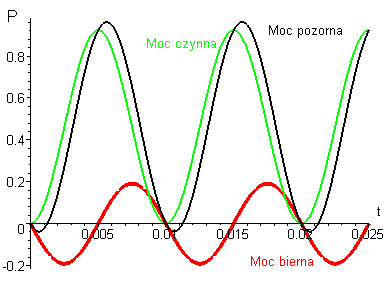
\includegraphics[scale=0.5]{power_types.png}
    \caption{Moc czynna, chwilowa i moc bierna podczas cykli zmian napięcia}
    \label{fig:my_label}
\end{figure}
\subsection{Współczynnik mocy czynnej do mocy pozornej}
Współczynnik mocy $cos{\varphi}$ - to stosunek mocy czynnej do mocy pozornej, czyli stosunek mocy użytecznej do iloczynu napięcia i prądu.
\begin{equation}
    cos(\varphi) = \frac{P}{S},
\end{equation}
\subsection{Harmoniczne prądu}
 Harmoniczna - jest napięciem lub prądem o wielokrotności częstotliwości podstawowej systemu energii elektrycznej, wytwarzanym przez działanie nieliniowych obciążeń, takich jak prostowniki, oświetlenie wyładowcze lub nasycone urządzenia magnetyczne. Częstotliwości harmoniczne w sieci energetycznej są częstą przyczyną problemów z jakością energii. Harmoniczne w systemach elektroenergetycznych powodują wzrost temperatury w urządzeniach i przewodach, przerwy w zapłonie w napędach o zmiennej prędkości oraz pulsacje momentu obrotowego w silnikach.
 \begin{figure}[H]
    \centering
    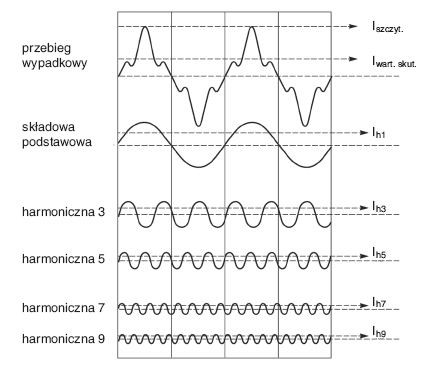
\includegraphics[scale=0.5]{harmonics}
    \caption{Analiza zjawiska odkształceń prądów i napięć}
    \label{fig:my_label}
\end{figure}
\section{Podstawowe pojęcia związane z komunikacją sieciową w modelu warstwowym TCP/IP}
\subsection{Adres IP}
Adres IP - jest to liczba nadawana interfejsowi sieciowemu w protokole IP, służąca identyfikacji elementów sieci w warstwie trzeciej modelu ISO/OSI.\\
IPv4 używa adresu 32 bitowego. Adres ten zapisuje się dziesiętnie oddzielając kolejne oktety kropkami. Na adres ten składają się dwa elementy: numer sieci oraz numer komputera w sieci, przy czym wielkość tych elementów może się zmieniać.\\
Przykładowy adres IPv4: \textit{192.168.1.10}
\subsection{Maska podsieci}
Maska podsieci pozwala na wyodrębnienie w adresie IP części będącej adresem podsieci i części, która jest adresem hosta w tej podsieci.\\
Podobnie jak adres IP, \textbf{maska podsieci} to również 32 bitowy ciąg, posiadający wartość 1 na pozycjach bitów odpowiadających numerowi sieci, a wartość 0 na pozycjach bitów odpowiadających numerowi urządzenia w sieci.\\
Przykładowa maska podsieci: \textit{255.255.255.0}
\subsection{Brama sieciowa}
Brama sieciowa - to maszyna podłączona do sieci komputerowej, za pośrednictwem której komputery z sieci lokalnej komunikują się z komputerami w innych sieciach.
\subsection{DHCP}
DHCP umożliwia podłączonym do sieci komputerom pobieranie adresu IP, maski podsieci, adresu bramy i serwera DNS oraz innych ustawień ze skonfigurowanej wcześniej puli adresów. Serwer DHCP może być skonfigurowany na osobnym komputerze i stanowił będzie osobne urządzenie w sieci przydzielające komputerom klienckim adresy IP, może również działać na już istniejącym serwerze jako osobna usługa, osobny proces.
\section{Protokół modbus TCP/IP}
\subsection{Komunikacja}
\textit{Modbus} jest protokołem komunikacyjnym działającym w modelu master-slave, który jest w stanie wspierać komunikację z 247 urządzeniami typu slave zorganizowanych  jako magistrala lub topologia gwiazdy. Komunikacja odbywa się w trybie half duplex.\\
\textbf{Modbus TCP/IP} jest protokołem Modbus wspierającym interfejs TCP działający w Ethernecie. Komunikacja sieciowa może być typu: pytanie-odpowiedź lub broadcastowa. \textit{Pytanie-odpowiedź} jest transmitowana z urządzenia typu master do nawiązanego połączenia z urządzeniem typu slave i po tym następuje wiadomość z odpowiedzią. \textit{Broadcast} jest transmitowany z urządzenia typu master do wszystkich urządzeń typu slave i po nim nie następuje odpowiedź.
Struktura przesyłania komunikatów Modbus to protokół aplikacji, który określa reguły organizowania i interpretowania danych niezależnie od nośnika transmisji danych. TCP/IP odnosi się do protokołu kontroli transmisji i protokołu internetowego, który zapewnia medium transmisyjne dla wiadomości Modbus TCP/IP. Mówiąc wprost, TCP/IP umożliwia wymianę bloków danych binarnych między komputerami. Jest to również światowy standard, który służy jako podstawa dla sieci WWW. Podstawową funkcją TCP jest zapewnienie, że wszystkie pakiety danych zostaną odebrane poprawnie, podczas gdy IP zapewnia, że wiadomości są poprawnie adresowane i kierowane. Zasadniczo komunikat Modbus TCP/IP to
po prostu komunikacja Modbus zamknięta w opakowaniu Ethernet TCP/IP.
W praktyce Modbus TCP osadza standardową ramkę danych Modbus w ramce TCP,
bez sumy kontrolnej Modbus, jak pokazano na poniższym schemacie.
\subsection{Ramka wiadomości}
Ramka wiadomości Modbus RTU składa się z następujących segmentów:
\begin{enumerate}
    \item \textbf{START FRAME}: znacznik rozpoczynający wiadomość
    \item \textbf{TRANSACTION ID}: pole identyfikacyjne służy do parowania transakcji, gdy wiele wiadomości jest wysyłanych wzdłuż tego samego połączenia TCP przez klienta bez oczekiwania na wcześniejszą odpowiedź
    \item \textbf{PROTOCOL ID}: to pole ma zawsze wartość 0 dla usług \textit{Modbus}, a inne wartości są zarezerwowane dla przyszłych rozszerzeń
    \item \textbf{LENGTH}: to pole jest liczbą bajtów pozostałych pól i obejmuje
bajt identyfikatora jednostki, bajt kodu funkcji i pola danych
    \item \textbf{UnitID}: to pole służy do identyfikacji zdalnego serwera zlokalizowanego w sieci innej niż TCP/IP (do mostkowania szeregowego).
    \item \textbf{ERROR CHECK}: pole uwzględniające kod korekcyjny (jednakże
pole sprawdzania błędów Modbus (suma kontrolna) nie jest używane jako standardowy TCP/IP w Ethernecie. Zamiast tego stosuje się metody sumy kontrolnej warstwy łącza danych w celu zagwarantowania integralności danych)
    \item \textbf{END OF FRAME}: znacznik kończący wiadomość
\end{enumerate}
%rysuneczek here :)))
\section{Przebieg laboratorium}
\subsection{Konfiguracja urządzeń}
Podczas laboratorium połączyliśmy bezpośrednio ze sobą komputer z analizatorem parametrów sieci EMA-90N kablem typu skręta zakończonym złączami RJ45.\\
Komputerowi nadaliśmy stały adres IP: \textbf{192.168.50.50}, natomiast analizatorowi \textbf{192.168.50.100}. Oba te adresy mają domyślną maskę podsieci: \textbf{255.255.255.0}. Komunikację między urządzeniami sprawdziliśmy wpierw za pomocą polecenia \textbf{ping} protokołu ICMP, a następnie za pomocą programu testowowego, który znajduje się pod adresem: \url{http://www.zsk.ict.pwr.wroc.pl/zsk/repository/dydaktyka/up/lab/analizator_sieci/ema90n_demo.zip} .
\subsection{Listing}
\begin{lstlisting}[language=c]
TcpClient client;
NetworkStream stream;
bool capture = false;
float activePowerCalcVal = 0;
int currentSleep = 0;

public Form1()
{
  InitializeComponent();
  client = new TcpClient("192.168.50.50", 502);
  stream = client.GetStream();
  Task.Run(async () => await CaptureProc());
}
private async Task CaptureProc()
{
  int sleep = 200;
  var voltageSeries = voltageChart.Series["voltageSeries"];
  using (StreamWriter file = File.CreateText("data.csv"))
  {
    file.WriteLine("time,voltage,current,cosfi,
    powerActive,powerActiveCalc,powerActiveDiff");
    while (true){
      if (capture){
        float blabla = currentSleep / 1000;
        string buff = blabla.ToString("0.00", System.Globalization.CultureInfo.InvariantCulture);
        float voltageVal = 
        readRegister(new byte[] { 0x10, 0x02 }) / 1000;
        voltage.Invoke(new Action(()
        => voltage.Text = voltageVal.ToString()));
        buff += voltageVal.ToString("0.00", System.Globalization.CultureInfo.InvariantCulture) + ",";
        float currentVal = 
        readRegister(new byte[] { 0x10, 0x10 }) / 100;
        current.Invoke(new Action(() 
        => current.Text = currentVal.ToString()));
        buff += currentVal.ToString("0.00", System.Globalization.CultureInfo.InvariantCulture) + ",";
        float cosfiVal = 
        readRegister(new byte[] { 0x10, 0x20 }) / 1000;
        cosfi.Invoke(new Action(() => cosfi.Text = cosfiVal.ToString()));
        buff += cosfiVal.ToString("0.00", System.Globalization.CultureInfo.InvariantCulture) + ",";
        float powerActiveVal = readRegister(new byte[] { 0x10, 0x30 });
        powerActive.Invoke(new Action(() => 
        powerActive.Text = powerActiveVal.ToString()));
        buff += powerActiveVal.ToString("0.00", System.Globalization.CultureInfo.InvariantCulture) + ",";
        activePowerCalcVal =
        Math.Abs(voltageVal * currentVal * cosfiVal) / 10;
        buff += activePowerCalcVal.ToString("0.00", System.Globalization.CultureInfo.InvariantCulture) + ",";
        float diff = Math.Abs(activePowerCalcVal - powerActiveVal);
        buff += diff.ToString("0.00", System.Globalization.CultureInfo.InvariantCulture);
        activePowerCalc.Invoke(new Action(() 
        => activePowerCalc.Text = activePowerCalcVal.ToString()));
        activePowerDiff.Invoke(new Action(() => 
        activePowerDiff.Text = diff.ToString()));
        file.WriteLine(buff);
        file.Flush();
        voltageChart.Invoke(new Action(() => {
          voltageChart.Series["voltageSeries"].Points.AddXY(currentSleep, voltageVal);
          voltageChart.Series["powerSeries"].Points.AddXY(currentSleep, powerActiveVal);
          voltageChart.Invalidate();
        }));
        currentSleep += 200;
        Thread.Sleep(sleep);
      }
    }
  }
}
private float readRegister(byte[] register) 
{
  byte[] request = { 0x00, 0x01, 0x00, 0x00, 0x00, 0x06, 0x01, 0x03, register[0], register[1], 0x00, 0x02 };
  stream.Write(request, 0, request.Length);
  byte[] answer = new byte[100];
  stream.Read(answer, 0, answer.Length);
  byte[] cut = new byte[4];
  Array.ConstrainedCopy(answer, 9, cut, 0, 4);
  Array.Reverse(cut);
  float value = BitConverter.ToInt32(cut, 0);
  return value;
}
private void button1_Click(object sender, EventArgs e)
{
  if (capture){
    capture = false;
    button1.Text = "Wlacz mierzonko";
    button1.BackColor = default(Color);
  } else{
    capture = true;
    button1.BackColor = Color.Red;
    button1.Text = "Wylacz mierzonko";
    voltage.Text = 0.ToString();
    current.Text = 0.ToString();
    currentSleep = 0;
    voltageChart.Invoke(new Action(() => {
      voltageChart.Series["voltageSeries"].Points.Clear();
      voltageChart.Series["powerSeries"].Points.Clear();
      voltageChart.Invalidate();
    }));
  }
}
\end{lstlisting}
\end{document}